\documentclass[25pt, a0paper, portrait]{tikzposter}
\tikzposterlatexaffectionproofoff
\usepackage[T1]{fontenc}
\usepackage[utf8]{inputenc}
\usepackage[australian]{babel}
\usepackage{csquotes}

\usetheme{Rays}

\usepackage[
	backend=biber,
	citestyle=authoryear,
	maxbibnames=99,
	maxnames=99
]{biblatex}
\addbibresource{poster.bib}

\usepackage{siunitx}

\usepackage{amsthm,amsfonts,amssymb,amsmath,mathtools,graphicx}

\renewcommand{\leq}{\leqslant}
\renewcommand{\geq}{\geqslant}

\title{Group Geodesic Growth}
\author{Alex Bishop}
%\date{\today}
\institute{University of Technology Sydney, Australia\\
	\vspace*{-6.5em}\hspace*{45cm}
\includegraphics{figure/profile.jpg}}

\begin{document}
	
	\maketitle
	
	\block{Introduction}{\Large
		Topics of regular group growth have been well studied; for example, Gromov's famous theorem that the groups of polynomial growth are precisely the virtually nilpotent ones, a corollary to which being that only polynomial growth of integer degree is possible; and Grigorchuk's proof of a group with intermediate regular growth.
		However, if these problems are slightly modified to instead count the number of shortest paths (geodesics) in a group, then all of these well-known results become open questions. 
	}
	
	\begin{columns}
		\column{0.475}
		
		\block{Def\textsuperscript{\,n}: Geodesic Growth} {\Large
			Given a group $G$ with finite symmetric generating set $X$, the \emph{geodesic growth function}, $\Gamma_{G,X}$, counts the geodesic word within a given length
			\[
			  \Gamma_{G,X} (n)
			  \coloneqq
			  \left\vert
			  \left\{
			    w = x_1 x_2 \cdots x_k \in X^\ast
			    \ \middle\vert\ 
			    \ell_X(w) = k \leq n
			  \right\}
			  \right\vert
			\]
			
			\medskip
			
			Then, given the regular growth function, $\gamma_{G,X}$, it is clear that
			\[
			  \gamma_{G,X}(n)
			  \leq
			  \Gamma_{G,X}(n)
			  \leq
			  \left\vert X \right\vert^{n+1}
			\]
		}
	
		\block{Example 2: Different Geodesic Growth Classes}{
			
			\vspace*{0.5em}
			
			\begin{minipage}{0.55\linewidth}
				\textbf{Presentation:}
				\[
					\left\langle
						a, t
					\ \middle\vert\
						t^2, [a,t]
					\right\rangle
				\]
				\vspace{0.5em}
			\end{minipage}
			~
			\begin{minipage}{0.45\linewidth}
				\begin{tikzfigure}
					\centering
					\includegraphics[page=1,width=\linewidth]{figure/z/figure2}
				\end{tikzfigure}
			\end{minipage}
			
			\vspace{-1.25em}
			
			\textbf{Geodesic Growth Rate:} \textit{polynomial}
			\[
				\Gamma_{\left\{ a^{\pm 1}, t \right\}}(n)
				=
				n^2+3n
				\quad
				\textit{(for }n \geq 2\textit{)}
			\]
			
			\vspace{1.5em}
			
			\begin{minipage}{0.55\linewidth}
					\textbf{Tietze Transform:} (where $c = at$)
					\[
					\left\langle
					a,c
					\ \middle\vert\ 
					a^2 = c^2,
					[a,c]
					\right\rangle
					\]
					\vspace{0.5em}
				\end{minipage}
				~
				\begin{minipage}{0.45\linewidth}
					\begin{tikzfigure}
						\centering
						\includegraphics[page=2,width=\linewidth]{figure/z/figure2}
					\end{tikzfigure}
			\end{minipage}
			
			\vspace{-1.25em}
			
			\textbf{Geodesic Growth Rate:} \textit{exponential}
			\[
				\Gamma_{\left\{ a^{\pm 1}, c^{\pm 1} \right\}}(n)
				=
				2^{n+1}-1
			\]
			
			\vspace*{0.5em}
		}
		
		\column{0.525}

		\block{Example 1: $\mathbb{Z}^2$}{
			\begin{minipage}{0.75\linewidth}
			\textbf{Presentation:}
				$
					\mathbb{Z}^2 =
					\left\langle
						a,b
					\,\middle\vert\,
						\left[ a,b \right]
					\right\rangle$
			
			\vspace*{1em}
			
			\begin{tabular}{l l c l}
				\textbf{Regular Growth:} &\textit{polynomial}
				&\ ---\ \ &
				$
				\gamma(n)
				=
				2n^2+2n+1
				$
				
				\\[1em]
				
				\textbf{Geodesic Growth:} &\textit{exponential}
				&\ ---\ \ &
				$
				\Gamma(n)
				=
				2^{n+3} - 4n - 7
				$
			\end{tabular}
			
			\end{minipage}
			~
			\begin{minipage}{0.2\linewidth}
				\begin{tikzfigure}
					\centering
					\includegraphics[width=\linewidth]{figure/z2/figure}
				\end{tikzfigure}
			\end{minipage}
		
			\vspace*{1em}
			
			\textbf{Proposition:} (\cite{OnGroupsPolynomial})
			
			\begin{center}
				$\mathbb{Z}^2$ has exponential geodesic growth with respect to every finite generating set
			\end{center}
		}
	
		\block{Example 3: Virtually $\mathbb{Z}^2$}{
			\textbf{Presentation:}
			$
				\left\langle
					a,b,t
				\,\middle\vert\,
					[a,b], t^2, a^t=b
				\right\rangle
			$
			
			\vspace{0.5em}
			
			\textbf{Geodesic Growth}: \textit{exponential} (it contains a $\mathbb{Z}^2$, see Example 1)
			\[
			\Gamma_{\left\{a^{\pm 1},b^{\pm 1},t\right\}}(n)
			=
			(n + 1)\cdot 2^{n + 2} - 2 n^2 - 6n - 2
			\qquad \textit{(for }n \geq 5\textit{)}
			\]
			
			\vspace{1em}
			
			\textbf{Remove $b$ by a Tietze Transform}:
			$
				\left\langle
					a,t
				\,\middle\vert\,
					\left[a,a^t\right], t^2
				\right\rangle
			$
			
			\vspace{0.5em}
			
			\textbf{Geodesic Growth}: \textit{polynomial} (compare this with Example 1)
			\[
			\Gamma_{\left\{a^{\pm 1},t \right\}} (n)
			=
			\left(2n^3 - 2n + 18\right)/3
			\qquad\qquad \textit{(for }n \geq 5\textit{)}
			\]
		}

	\end{columns}
	
	\block{Main Question}{\bfseries\Huge\centering
		\vspace*{0.5em}
		
		Does there exist a group with intermediate geodesic growth?
		
		\vspace*{0.5em}
	}
	
	\begin{columns}
		\column{0.55}
		
		\block{How about Grigorchuk's Group?}{
			Consider the $n$\textsuperscript{th} level Schreier Graphs
			
			\vspace*{1em}
			
			\begin{tikzfigure}[4\textsuperscript{th} level Schreier graph]
				\centering
				\includegraphics[width=\linewidth,page=5]{figure/grig/schreier}
			\end{tikzfigure}
		
			\vspace*{1em}
		
			\textbf{Anwser}: exponential --- There are exponentially many geodesics in the Schreier graphs, which are also geodesics of the group.
		}
	
		\block{Experimental Mathematics}{
			Results of a computer enumeration of geodesics (of the Gupta-Fabrykowski group):
			
			\begin{tikzfigure}
				\centering
				
				%%%%%%%%%%%%%%%%%%%%%%%%%%%%%%%%%%%%%%%%%%%%%%%
				
				\begin{minipage}{0.2\linewidth}
				\end{minipage}
				~
				\begin{minipage}{0.2\linewidth}
					\centering
					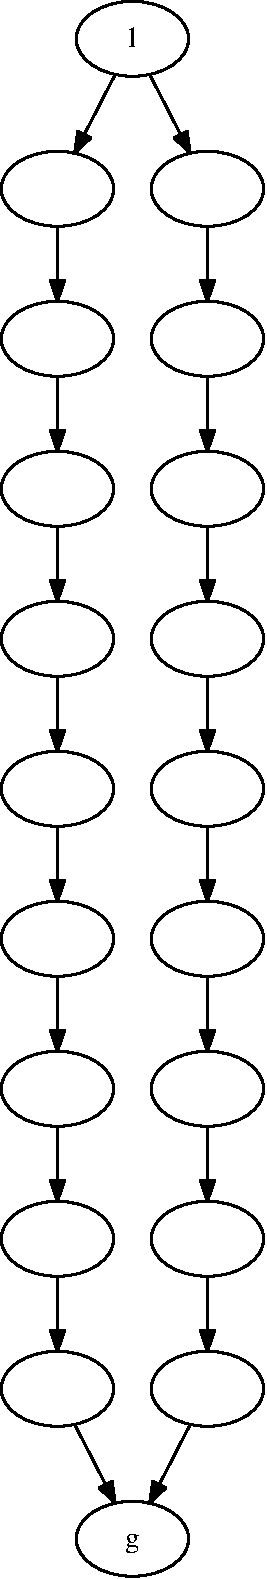
\includegraphics[height=14cm]{figure/patterns/pattern1}
				\end{minipage}
				~
				\begin{minipage}{0.2\linewidth}
					\centering
					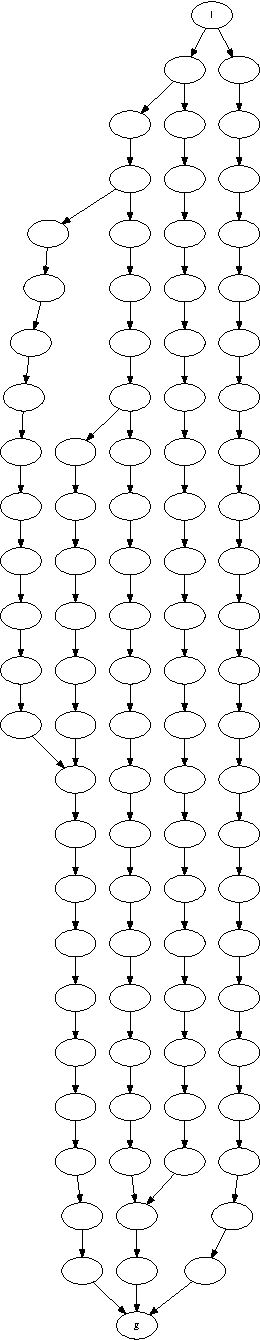
\includegraphics[height=14cm]{figure/patterns/pattern2}
				\end{minipage}
				~
				\begin{minipage}{0.2\linewidth}
					\centering
					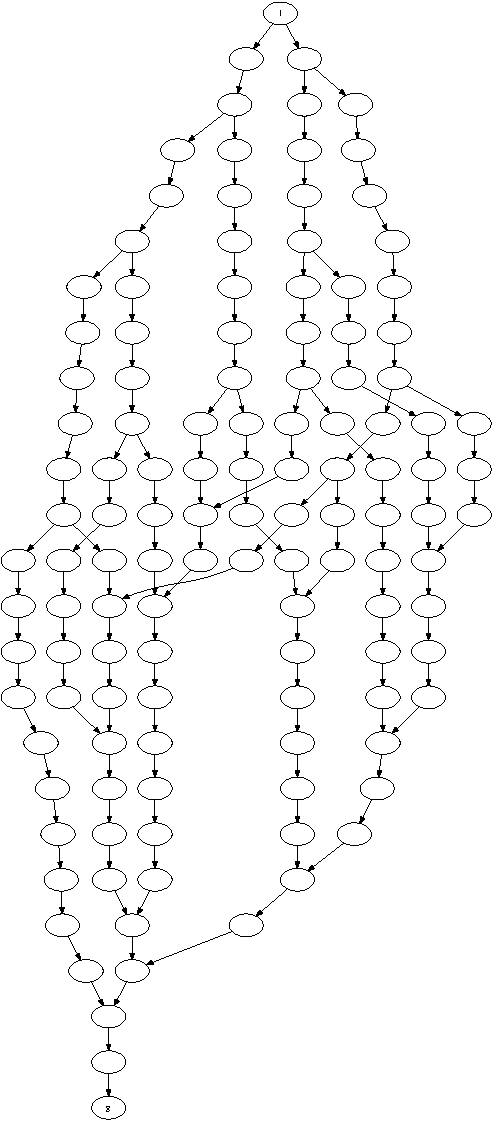
\includegraphics[height=14cm]{figure/patterns/pattern3}
				\end{minipage}
				
				
				%%%%%%%%%%%%%%%%%%%%%%%%%%%%%%%%%%%%%%%%%%%%%%%
				
			\end{tikzfigure}
		
%			Above are sub-graphs of the Cayley graph of the Gupta-Fabrykowski group
		}
	
		\column{0.45}
		
		\block{What about groups similar to Grigorchuk's?}{
		
			Following the idea of considering the Schreier graphs \citeauthor{Julie2016GeodesicGrowth} showed
	
			\vspace*{1em}
	
			\begin{tabular}{c r l}
				&\textbf{Grigorchuk $G_\omega$}:&
				exponentially many geodesics
				\\[0.5em]
				&\textbf{Gupta-Sidki $p$-groups}:&
				exponentially many geodesics
				\\[0.5em]
				&\textbf{Square group}:&
				exponentially many geodesics
				\\[0.5em]
				&\textbf{Spinal group}:&
				exponentially many geodesics
				\\[0.5em]
				&\color{red}\textbf{Gupta-Fabrykowski}: &
				\color{red} technique is inconclusive; unkown if exponential
			\end{tabular}
		
		\vspace*{1em}
		
		\textbf{Proposition}: (\cite{PolynomialSchreier})
		
		\medskip\medskip
		
		\addtolength{\leftskip}{1em}
		
		There are only polynomially many (of degree $\log_2 3$) geodesics in the level Schreier graphs  of the Gupta-Fabrykowski group
	
		}
	
		\block{Potential Techniques}{
			Given a particular group of intermediate regular growth:
			
			\vspace*{0.5em}
			
			\begin{itemize}
				\item
				Consider the function which counts the number of geodesics per element.
				If this function has a sub-exponential upper bound with respect to the word length then we have intermediate geodesic growth
				
				\vspace{0.5em}
				
				\item
				Consider different generating sets e.g.\@ does Grigorchuk's group have exponential geodesic growth with respect to every generating set?
				
				\vspace{0.5em}
				
				\item
				Attempt to find a convenient formal language which includes all the geodesics.
			
			\end{itemize}
		
		\vspace{0.5em}
		
			\emph{or} attempt to cosntruct a virtually nilpotent group with the desired property
		}
	
%\block{References}{
%\printbibliography[heading=none]
%}
%	\block{Schreier Graph for Fabrykowski-Gupta}
%{\Large
%
%\begin{tikzfigure}[the 6\textsuperscript{th} level Schreier graph \cite{Julie2016GeodesicGrowth}]
%	\centering
%	\includegraphics[width=0.4\linewidth]{figure/schreier}
%\end{tikzfigure}
%}
	\end{columns}
	
\end{document}